\documentclass{standalone}

\usepackage{ctex}
\usepackage{van-de-la-sehen}
\DeclareMathOperator{\Mathieuce}{ce}
\DeclareMathOperator{\Mathieuse}{se}
\DeclareMathOperator{\MathieuCe}{Ce}
\DeclareMathOperator{\MathieuSe}{Se}

\def\externallinksymbol{\raisebox{-.2\height}{\includegraphics[width=.9em]{externallink.eps}}}
\let\oldhref\href
\def\href{\externallinksymbol\oldhref}

\begin{document}

\begin{tabular}{>{\centering}m{2cm}>{\centering}m{2cm}% titles end
>{\centering}m{6cm}>{\centering}m{11cm}>{\centering}m{11cm}>{\centering\arraybackslash}m{11cm}% planar end
>{\centering\arraybackslash}m{9cm}>{\centering\arraybackslash}m{17cm}>{\centering\arraybackslash}m{17cm}% three dimensional end
}
    \toprule
    \+:m22{c}{坐标系} & \+:c4{c}{平面} & \+:c2{c}{三维} \\
    & & \+:c1{c}{一般} & \+:c1{c}{椭圆坐标系} & \+:c1{c}{抛物线坐标系} & \+:c1{c}{双极坐标系} & \+:c1{c}{一般} & \+:c1{c}{扁球面坐标系} & \+:c1{c}{圆环坐标系}  \\
    \midrule
    %
    \+:c2{c}{宗量} & \+:c1{c}{$\pare{\mu,\nu}$} & \+:c1{c}{$\pare{\mu, \nu}$} & \+:c1{c}{$\pare{\sigma, \tau}$} & \+:c1{c}{$\pare{\mu,\nu}$} & & \+:c{1}{c}{$\pare{\mu,\nu,\varphi}$} & \+:c{1}{c}{$\pare{\sigma,\tau,\varphi}$} \\
    \midrule
    %
    \+:m42{c}{宗量诠释} & 参量 & %
    {$\pare{\pm a,0}$是坐标曲线中椭圆和双曲线的共有焦点} & & %
    {$\pare{\pm a,0}$是确定圆族的一对对称点, $F_1$和$F_2$} & %
    & %
    {$\pare{\pm a,0}$是坐标曲面中椭球和双曲面的共有焦点} & %
    {$\pare{\pm a,0}$是确定圆族的一对对称点, $F_1$和$F_2$} \\
    \cmidrule{3-9}
    & & $\mu$ & {$a\cosh\mu$是坐标曲线中椭圆的半长轴} & %
    {$\sigma^2$是开口朝上抛物线的焦点到焦线的距离} & %
    $\displaystyle \sigma = \angle F_1PF_2 $ & %
    & %
    $a\cosh\mu$是坐标曲面中椭球的半长轴 &%
    $\displaystyle \sigma = \angle F_1PF_2 $ \\
    \cmidrule{3-9}
    & & $\nu$ & %
    {$a\cos\nu$是坐标曲线中双曲线的半横轴} & %
    {$\tau^2$是开口朝下抛物线的焦点到焦线的距离} & %
    $\displaystyle \tau = \ln \frac{\abs{F_1P}}{\abs{F_2P}} $ & %
    & %
    {$a\cos\nu$是坐标曲面中双曲面的半横轴} & %
    $ \displaystyle \tau = \ln \frac{\abs{F_1P}}{\abs{F_2P}} $  \\
    \cmidrule{3-9}
     & &%
    \+:c4{c}{N/A} & & %
    $\varphi$表示经度 & %
    $\varphi$表示经度 \\
    \midrule
    %
    \+:c2{c}{示意图} & & %
    {\includegraphics{src_plot/Elliptic.pdf}} & %
    {\includegraphics{src_plot/Parabolic.pdf}} & %
    {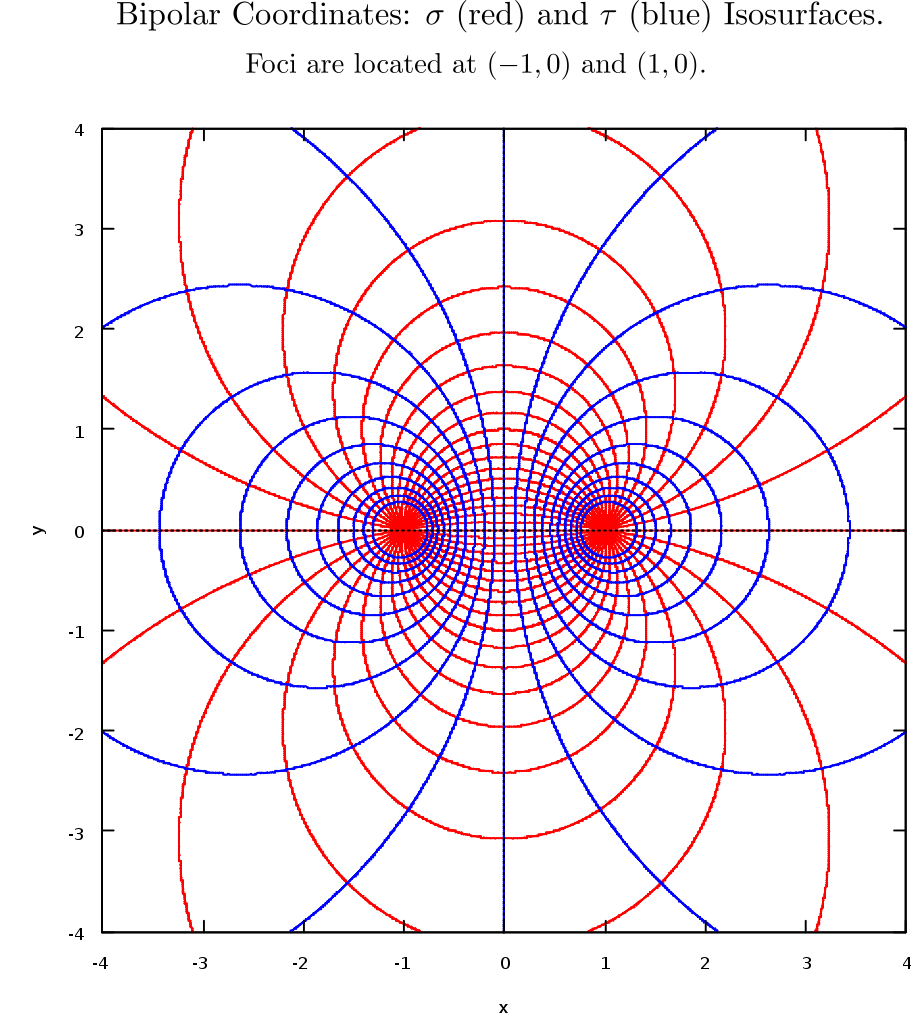
\includegraphics{src_plot/Bipolar.pdf}} \\ %
    \midrule
    %
    \+:c2{c}{坐标变换} & %
    {%
        $\displaystyle \left\{\begin{aligned}
            x &= x\pare{\mu,\nu}, \\
            y &= y\pare{\mu,\nu}.
        \end{aligned}\right. $%
    }& %
    {%
        $\displaystyle \left\{\begin{aligned}
            x &= a\cosh \mu \cos \nu, \\
            y &= a\sinh \mu \sin \nu.
        \end{aligned}\right. $%
    } & %
    {%
        $\displaystyle \left\{\begin{aligned}
            x &= \pm \sigma\tau, \\
            y &= \half\pare{\tau^2 - \sigma^2}.
        \end{aligned}\right.  $%
    } & %
    {%
        $\displaystyle \left\{\begin{aligned}
            x &= a \frac{\sinh \tau}{\cosh \tau - \cos\sigma}, \\
            y &= a \frac{\sin\sigma}{\cosh\tau - \cos\sigma}.
        \end{aligned}\right. $%
    } & %
    & %
    {%
        $\displaystyle \left\{\begin{aligned}
            x &= a\cosh \mu \cos \nu \cos\varphi, \\
            y &= a\cosh \mu \cos \nu \sin\varphi, \\
            z &= a\sinh \mu \sin \nu.
        \end{aligned}\right. $%
    } & %
    {%
        $\displaystyle \left\{\begin{aligned}
            x &= a \frac{\sinh \tau}{\cosh \tau - \cos\sigma}\cos\varphi, \\
            y &= a \frac{\sinh \tau}{\cosh \tau - \cos\sigma}\sin\varphi, \\
            z &= a \frac{\sin\sigma}{\cosh\tau - \cos\sigma}.
        \end{aligned}\right. $%
    } \\%
    \midrule
    %
    \+:c2{c}{生成变换} & & %
    {$\displaystyle z = a\cosh w $} & %
    {$\displaystyle z = \frac{w^2}{2} $} & %
    {$\displaystyle z = ai\cot\pare{\frac{w}{2}} $} & %
    & %
    椭圆坐标系绕两焦点的中垂线旋转 & %
    双极坐标系绕两极点的中垂线旋转 \\
    \midrule
    %
    \+:r3{度规} & %
    $h_1$ & %
    $\displaystyle \sqrt{g_{11}} = \sqrt{\pare{\+D{\mu}Dx}^2+\pare{\+D{\mu}Dy}^2} $ &  %
    \+:r3{$\displaystyle a\sqrt{\sinh^2\mu + \sin^2\nu} $} & %
    \+:r3{$\displaystyle \sqrt{\sigma^2 + \tau^2} $} & %
    \+:r3{$\displaystyle \frac{a}{\cosh\tau - \cos\sigma} $} & %
    & %
    \+:r3{$\displaystyle a\sqrt{\sinh^2\mu + \sin^2\nu} $} & %
    \+:r3{$\displaystyle \frac{a}{\cosh\tau - \cos\sigma} $} \\
    \cmidrule{3-3}
    & $h_2$ & %
    $\displaystyle \sqrt{g_{22}} = \sqrt{\pare{\+D{\nu}Dx}^2+\pare{\+D{\nu}Dy}^2} $ & & & \\
    \cmidrule{3-9}
    & $h_3$ & \+:c4{c}{N/A} & & %
    $\displaystyle a\cosh\mu\cos\nu$ & %
    $\displaystyle \frac{a\sinh \tau}{\cosh\tau - \cos\sigma}$ \\
    \midrule
    %
    \+:c2{c}{体元} & %
    $\displaystyle \rd{A} = h_1 h_2 \,\rd{\mu}\,\rd{\nu} $ & %
    $\displaystyle \rd{A} = a^2\pare{\sinh^2\mu + \sin^2\nu}\,\rd{\mu}\,\rd{\nu} $ & %
    $\displaystyle \rd{A} = \pare{\sigma^2 + \tau^2}\,\rd{\sigma}\,\rd{\tau} $  &
    $\displaystyle \rd{A} = \pare{\frac{a}{\cosh\tau - \cos\sigma}}^2\,\rd{\mu}\,\rd{\nu} $ \\
    %
    \midrule
    \+:r4{微分} & $\grad\Phi$ & %
    $\displaystyle \sum_k \frac{\+ue_k}{h_k}\+D{q^k}D{\Phi}$ & %
     & %
     & %
     \\
    \cmidrule{3-9}
    & $\div\+vF$ & %
    $\displaystyle \sum_k \rec{H}\+D{q^k}D{}\pare{\frac{H}{h_k}F_k}$ & %
     & %
     & %
     \\
    \cmidrule{3-9}
    & $\curl\+vF$ & %
    %$\displaystyle \sum_{ijk} \frac{h_k\+ue_k}{H}\epsilon_{ijk}\+D{q^i}D{}\pare{h_jF_j}$
    \+:c4{c}{N/A}
    \\
    \cmidrule{3-9}
    & $\laplacian\Phi$ &
    $\displaystyle \sum_k \rec{H}\+D{q^k}D{}\pare{\frac{H}{h_k^2}D{q^k}D{\Phi}}$ & %
    $\displaystyle \rec{a^2\pare{\sinh^2\mu + \sin^2\nu}}\pare{\frac{\partial^2\Phi}{\partial \mu^2} + \frac{\partial^2\Phi}{\partial\nu^2}}$ & %
    $\displaystyle \rec{\sigma^2 + \tau^2} \pare{\frac{\partial^2\Phi}{\partial \sigma^2} + \frac{\partial^2\Phi}{\partial\tau^2}}$ & %
    $\displaystyle \pare{\frac{\cosh \tau - \cos\sigma}{a}}^2 \pare{\frac{\partial^2\Phi}{\partial \sigma^2} + \frac{\partial^2\Phi}{\partial\tau^2}}$ & %
    & %
    $\displaystyle \rec{a^2\pare{\sinh^2 \mu + \sin^2\nu}} \brac{ \rec{\cosh\mu}\+D\mu D{}\pare{\cosh\mu \+D\mu D\Phi} + \rec{\cos\nu}\+D\nu D{}\pare{\cos\nu \+D\nu D\Phi} } + \rec{a^2\pare{\cosh^2\mu \cos^2\nu}}\frac{\partial^2\Phi}{\partial\varphi^2}$ & %
    $\displaystyle \frac{\pare{\cosh\tau - \cos\sigma}^2}{a^2\sinh\tau}\brac{ \+D\sigma D{}\pare{\frac{\sinh\tau}{\cosh\tau - \cos\sigma}\+D\sigma D\Phi} + \+D\tau D{}\pare{\frac{\sinh\tau}{\cosh\tau - \cos\sigma}\+D\tau D\Phi} + \rec{\sinh\tau\pare{\cosh\tau - \cos\sigma}} \frac{\partial ^2\Phi}{\partial \varphi^2} }$ \\
    %
    \midrule
    \+:c2{c}{Laplace方程基本解} & %
    $\displaystyle \laplacian F\pare{\mu}G\pare{\nu} = 0$ & % 
    \+:r4{$\displaystyle \begin{cases}
        \MathieuCe_n\pare{\mu,q}\Mathieuce_n\pare{\nu,q}, \\
        \MathieuSe_n\pare{\mu,q}\Mathieuse_n\pare{\nu,q},
    \end{cases}\quad q = \frac{c^2k^2}{2}.$} & & & & %
    & %
    $\displaystyle \begin{cases}
        S_\nu\pare{\sigma} = e^{\pm i\nu\sigma}, \\
        T_{\mu\nu}\pare{\tau} = P^{\mu}_{\nu-1/2}\pare{\cosh \tau},\ Q^{\mu}_{\nu-1/2}\pare{\cosh\tau}, \\
        V_\mu\pare{\varphi} = e^{\pm i\mu\varphi}.
    \end{cases}$ \\
    \cmidrule{9-9}
    \+:c2{c}{Helmholtz方程基本解} & %
    $\displaystyle \laplacian F\pare{\mu}G\pare{\nu} + k^2 F\pare{\mu}G\pare{\nu} = 0$ & & & & & %
    & %
    \href{http://mathworld.wolfram.com/HelmholtzDifferentialEquationToroidalCoordinates.html}{N/A} \\
    \midrule
     \\
    \bottomrule
\end{tabular}

\end{document}
